% \documentclass[a4paper, conference, compsoc]{IEEEtran}
\documentclass[12pt,a4paper,colorinlistoftodos]{article}
% \documentclass[%
%     pdftex,
%     oneside,			% Einseitiger Druck.
%     12pt,				% Schriftgroesse
%     parskip=half,		% Halbe Zeile Abstand zwischen Absätzen.
% %	topmargin = 10pt,	% Abstand Seitenrand (Std:1in) zu Kopfzeile [laut log: unused]
%     headheight = 12pt,	% Höhe der Kopfzeile
% %	headsep = 30pt,	% Abstand zwischen Kopfzeile und Text Body  [laut log: unused]
%     headsepline,		% Linie nach Kopfzeile.
%     footsepline,		% Linie vor Fusszeile.
%     footheight = 16pt,	% Höhe der Fusszeile
%     abstracton,		% Abstract Überschriften
%     DIV=calc,		% Satzspiegel berechnen
%     BCOR=8mm,		% Bindekorrektur links: 8mm
%     headinclude=false,	% Kopfzeile nicht in den Satzspiegel einbeziehen
%     footinclude=false,	% Fußzeile nicht in den Satzspiegel einbeziehen
%     listof=totoc,		% Abbildungs-/ Tabellenverzeichnis im Inhaltsverzeichnis darstellen
%     toc=bibliography,	% Literaturverzeichnis im Inhaltsverzeichnis darstellen
% ]{scrreprt}	% Koma-Script report-Klasse, fuer laengere Bachelorarbeiten alternativ auch: scrbook


% Basic packages
\usepackage[T1]{fontenc}
\usepackage[utf8]{inputenc}
\usepackage[scaled]{beramono}
\usepackage[english,ngerman]{babel,varioref}
\usepackage{xcolor}
\usepackage{amsmath}

% Tables
\usepackage{booktabs}
\usepackage{multirow}
\usepackage{longtable}
% Graphics and Includes
\usepackage[pdftex]{graphicx}
\graphicspath{{assets/img/}}
\DeclareGraphicsExtensions{.pdf,.jpeg,.png,.jpg}
\usepackage{tikz}
\usetikzlibrary{arrows.meta,bending,automata,shapes}
\usepackage[underline=true,rounded corners=false]{pgf-umlsd}

% Reduce distance before caption
\usepackage[skip=5pt]{caption}
\captionsetup[table]{position=below,skip=-5pt}
% Bibliography
\usepackage[backend=biber, isbn=false, doi=false, style=ieee]{biblatex}
\addbibresource{bibliography.bib}
\AtBeginBibliography{\raggedright}
%\nocite{*}

% Gossar z.a. für acronyme
% \usepackage[acronym]{glossaries}
% \makeglossaries
\usepackage[printonlyused]{acronym} % falls gewünscht kann die Option footnote eingefügt werden, dann wird die Erklärung nicht inline sondern in einer Fußnote dargestellt

% \section*{Abkürzungsverzeichnis}
\begin{acronym}[AAAAAAA]
    \acro{wysiwyg}[WYSIWYG]{What you see is what you get}
\end{acronym}

% Colors
\definecolor{ListingBackground}{HTML}{E6E6E6}
\definecolor{LinkColor}{HTML}{000000}


% Font
\usepackage[onehalfspacing]{setspace}
\usepackage{lmodern}
\usepackage[official]{eurosym}
\usepackage{enumitem}
\usepackage[locale=DE]{siunitx} % SI Units für Währungen
\DeclareSIUnit{\EUR}{\text{\euro}} % Beispielverwendung: \SI{10.10}{\EUR}

\usepackage[autostyle=true,german=quotes]{csquotes}
\usepackage{url}
\newcommand{\code}[1]{\texttt{#1}}

\newcommand{\reducedstrut}{\vrule width 0pt height .9\ht\strutbox depth .9\dp\strutbox\relax}
\newcommand{\highlight}[2]{
  \begingroup
  \setlength{\fboxsep}{0pt}
  \colorbox{#1}{\reducedstrut#2\/}
  \endgroup
}

% Additional Setup
\usepackage[unicode=true,hypertexnames=false,colorlinks=true,linkcolor=LinkColor,citecolor=LinkColor,urlcolor=LinkColor,pdftex]{hyperref}

% Trennung von URLs im Literaturverzeichnis (große Werte [> 10000] verhindern die Trennung)
\defcounter{biburlnumpenalty}{10} % Strafe für Trennung in URL nach Zahl
\defcounter{biburlucpenalty}{500}  % Strafe für Trennung in URL nach Großbuchstaben
\defcounter{biburllcpenalty}{500}  % Strafe für Trennung in URL nach Kleinbuchstaben
\interfootnotelinepenalty=10000 % prevent all footnotes from breaking over a page.

% Configs
\setcounter{tocdepth}{1} % Limit table of contents to subsection
\sisetup{detect-weight=true, detect-family=true} % SI Units shall detect font weight and family
\setlist[description]{style=nextline} % Break definitions of terms to a new line (used by \begin{description} \item[foo] bar \end{description})
\renewcommand*{\bibfont}{\small}

%Hurenkinder und Schusterjungen vermeiden
\clubpenalty = 10000
\widowpenalty = 10000
\displaywidowpenalty = 10000

% Quellcode
\usepackage{listings}
\usepackage{float}
\usepackage{textcomp}
\lstset{
    inputpath=assets/listings,
    language=Java,			% Standardsprache des Quellcodes
    numbers=left,			% Zeilennummern links
    stepnumber=1,			% Jede Zeile nummerieren.
    numbersep=5pt,			% 5pt Abstand zum Quellcode
    numberstyle=\tiny,		% Zeichengrösse 'tiny' für die Nummern.
    breaklines=true,		% Zeilen umbrechen wenn notwendig.
    breakautoindent=true,	% Nach dem Zeilenumbruch Zeile einrücken.
    postbreak=\space,		% Bei Leerzeichen umbrechen.
    tabsize=2,				% Tabulatorgrösse 2
    basicstyle=\ttfamily\footnotesize, % Nichtproportionale Schrift, klein für den Quellcode
    showspaces=false,		% Leerzeichen nicht anzeigen.
    showstringspaces=false,	% Leerzeichen auch in Strings ('') nicht anzeigen.
    extendedchars=true,		% Alle Zeichen vom Latin1 Zeichensatz anzeigen.
    captionpos=b,			% sets the caption-position to bottom
    backgroundcolor=\color{ListingBackground}, % Hintergrundfarbe des Quellcodes setzen.
    xleftmargin=0pt,		% Rand links
    xrightmargin=0pt,		% Rand rechts
    frame=single,			% Rahmen an
    frameround=ffff,
    rulecolor=\color{darkgray},	% Rahmenfarbe
    fillcolor=\color{ListingBackground},
    keywordstyle=\color[rgb]{0.133,0.133,0.6},
    commentstyle=\color[rgb]{0.133,0.545,0.133},
    stringstyle=\color[rgb]{0.627,0.126,0.941},
    float,
    upquote=true
}


\colorlet{punct}{red!60!black}
\definecolor{delim}{RGB}{20,105,176}
\colorlet{numb}{magenta!60!black}

\lstdefinelanguage{json}{
    string=[s]{"}{"},
    stringstyle=\color{numb},
    literate=
     *{0}{{{\color{numb}0}}}{1}
      {1}{{{\color{numb}1}}}{1}
      {2}{{{\color{numb}2}}}{1}
      {3}{{{\color{numb}3}}}{1}
      {4}{{{\color{numb}4}}}{1}
      {5}{{{\color{numb}5}}}{1}
      {6}{{{\color{numb}6}}}{1}
      {7}{{{\color{numb}7}}}{1}
      {8}{{{\color{numb}8}}}{1}
      {9}{{{\color{numb}9}}}{1}
      {:}{{{\color{punct}{:}}}}{1}
      {,}{{{\color{punct}{,}}}}{1}
      {\{}{{{\color{delim}{\{}}}}{1}
      {\}}{{{\color{delim}{\}}}}}{1}
      {[}{{{\color{delim}{[}}}}{1}
      {]}{{{\color{delim}{]}}}}{1}
}

\lstdefinelanguage{yaml}{
  identifierstyle=\color{delim},
  sensitive=false,
  comment=[l]{\#},
  commentstyle=\color{purple}\ttfamily,
  stringstyle=\color{numb},
  morestring=[b]',
  morestring=[b]"
}

\lstloadlanguages{Python,Java,bash}
% Useful tools
\usepackage{blindtext}
\usepackage{lipsum}
\usepackage[section]{placeins} % Prevent figures and tables to float to new section
\usepackage[obeyFinal,backgroundcolor=yellow,linecolor=black]{todonotes}


%Angaben zur Arbeit
\def\myTitel{Ein ansprechender Titel}
\def\myArbeit{Seminararbeit}
\def\myFach{Spanndendes Fach}
\def\myDatum{\today}
\def\myBetreuer{Netter Betreuer}
\def\myGutachter{Strenger Gutachter}
\def\myBearbeitungszeit{Lange}
\def\myAbgabeort{Heilbronn}

%Angaben zur Person
\def\myAutor{Wunderbarer Autor}
\def\myDegree{Master Informatik}
\def\myInstitution{DHBW CAS, Bildungscampus 13, 74076 Heilbronn}
\def\myMatrikelnr{123456}
\def\myKurs{TMINF17}
\def\myFirma{SAP SE}
\def\myFirmenort{Walldorf}
%\section*{Abkürzungsverzeichnis}
\begin{acronym}[AAAAAAA]
    \acro{wysiwyg}[WYSIWYG]{What you see is what you get}
\end{acronym}

\begin{document}


\title{\myTitel}
\author{\myAutor~(\myMatrikelnr)\\
    \small{\myFach}\\
    \small{\myDegree}\\
    \small{\myInstitution}
}
\date{\myDatum}

\begin{titlepage}
	\begin{longtable}{p{8.2cm} p{5.4cm}}
		% Firmenlogo
		&
		
\includegraphics[width=5.4cm]{casLogo}
	\end{longtable}
	\addtocounter{table}{-1}
    {\let\newpage\relax\maketitle}
    \thispagestyle{empty}
    % \vfill
    \begin{abstract}
    \lipsum[66]
\end{abstract}
\end{titlepage}
% \begin{titlepage}
	\begin{longtable}{p{8.2cm} p{5.4cm}}
		% Firmenlogo
		&
		
\includegraphics[width=5.4cm]{casLogo}
	\end{longtable}
	\addtocounter{table}{-1}
	\enlargethispage{20mm}
	\begin{center}
		\vspace*{12mm}	{\LARGE\textbf \myTitel }\\
		\vspace*{12mm}	{\large\textbf \myArbeit}\\
		% \vspace*{12mm}	\langdeckblattabschlusshinleitung\\
		\vspace*{3mm}		{\textbf \myDegree}\\
		\vspace*{12mm}	des Studiengangs \myKurs\\
    \vspace*{3mm}		am DHBW CAS\\
		\vspace*{12mm}	von\\
		\vspace*{3mm}		{\large\textbf \myAutor}\\
		\vspace*{12mm}	\myDatum\\
	\end{center}
	\vfill
	\begin{spacing}{1.2}
	\begin{tabbing}
		mmmmmmmmmmmmmmmmmmmmmmmmmm             \= \kill
		\textbf{Bearbeitungszeit}       \>  \myBearbeitungszeit\\
		\textbf{Matrikelnummer, Kurs}  \>  \myMatrikelnr, \myKurs\\
		\textbf{Firma}                  \>  \myFirma, \myFirmenort\\
		\textbf{Betreuer}               \>  \myBetreuer\\
		\textbf{Gutachter}              \>  \myGutachter
	\end{tabbing}
	\end{spacing}
\end{titlepage}

\pagenumbering{Roman}

% Sperrvermerk
% \thispagestyle{empty}
% Sperrvermerk direkt hinter Titelseite
\section*{Sperrvermerk}

\vspace*{2em}

Die vorliegende {\myArbeit} mit dem Titel {\itshape{} \myTitel{}\/}
enthält unternehmensinterne bzw. vertrauliche Informationen der {\myFirma},
ist deshalb mit einem Sperrvermerk versehen
und wird ausschließlich zu Prüfungszwecken am Studiengang
{\myDegree} der Dualen Hochschule Baden-Württemberg vorgelegt.
Sie ist ausschließlich zur Einsicht durch den zugeteilten Gutachter,
die Leitung des Studiengangs und ggf. den Prüfungsausschuss des Studiengangs
bestimmt.  Es ist untersagt,
\begin{itemize}
\item den Inhalt dieser Arbeit (einschließlich Daten, Abbildungen, Tabellen, Zeichnungen usw.) als Ganzes oder auszugsweise weiterzugeben,
\item Kopien oder Abschriften dieser Arbeit (einschließlich Daten, Abbildungen, Tabellen, Zeichnungen usw.) als Ganzes oder in Auszügen anzufertigen,
\item diese Arbeit zu veröffentlichen bzw. digital, elektronisch oder virtuell zur Verfügung zu stellen.
\end{itemize}
Jede anderweitige Einsichtnahme und Veröffentlichung – auch von Teilen der Arbeit – bedarf der vorherigen Zustimmung durch den Verfasser und {\myFirma}.

\vspace{3em}

\myAbgabeort, \myDatum
\vspace{4em}

\rule{6cm}{0.4pt}\\
\myAutor

% \newpage

% Erklärung
\thispagestyle{empty}

\section*{Selbstständigkeitserklärung}
\vspace*{2em}


Ich versichere hiermit, dass ich meinen {\myArbeit} mit dem Thema: {\itshape \myTitel } selbstständig verfasst und keine anderen als die angegebenen Quellen und Hilfsmittel benutzt habe. Ich versichere zudem, dass die eingereichte elektronische Fassung mit der gedruckten Fassung übereinstimmt.


\vspace{3em}
\noindent
\myAbgabeort, \myDatum
\\
\\
\noindent
\rule{6cm}{0.4pt}\\
\myAutor

\newpage


% \begin{abstract}
    \lipsum[66]
\end{abstract}
% \newpage

\pagestyle{plain}		% nur Seitenzahlen im Fuß

% Inhaltsverzeichnis
\begin{spacing}{1.1}
    \begingroup
        \pagestyle{empty}
        %für die Anzeige von Unterkapiteln im Inhaltsverzeichnis
        \setcounter{tocdepth}{2}

        \tableofcontents
        \clearpage
    \endgroup
\end{spacing}
\newpage

% Abkürzungsverzeichnis
% \cleardoublepage
% \section*{Abkürzungsverzeichnis}
\begin{acronym}[AAAAAAA]
    \acro{wysiwyg}[WYSIWYG]{What you see is what you get}
\end{acronym}


% Abbildungsverzeichnis
\cleardoublepage
\listoffigures

%Tabellenverzeichnis
\listoftables
\cleardoublepage

% Quellcodeverzeichnis
% \lstlistoflistings
% \cleardoublepage

% \listoftodos
% \cleardoublepage

\pagenumbering{arabic}

\section{Einleitung}\label{sec:einleitung}
Ohne Blutspenden wäre die moderne Medizin undenkbar.
Sei es für die Behandlung von Krebs- und Herzerkrankungen,
für die Unfallchirurgie oder für andere medizinische Eingriffe.
Täglich werden deutschlandweit circa 15.000 Blutspenden benötigt. \cite{FragenAn98:online}

Deshalb bietet das Deutsche Rote Kreuz regelmäßig in verschiedenen Orten und Gemeinden die Möglichkeit an Blut zu spenden.
Diese Spende ist aus gesundheitlichen Gründen jedoch nur unter bestimmten Bedingungen gestattet.
Hierzu zählen unter anderem \cite{SpendeCh65:online}:
\begin{itemize}
    \setlength\itemsep{-0.5em}
    \item Alter zwischen 18 und 65 Jahre
    \item Mindestgewicht 50 kg
    \item Kein Arzttermin innerhalb der vergangenen 7 Tage
    \item Keine Operationen innerhalb von 12 Monaten
\end{itemize}

Bei diesen Bedingungen hat der anwesende Arzt einen gewissen Ermessenspielraum und kann eine Spende dennoch genehmigen.
Es gibt jedoch auch \enquote{harte} Bedingungen, welche eine Spende ausschließen können:

\begin{itemize}
    \setlength\itemsep{-0.5em}
    \item Keine Spende innerhalb der letzten 56 Tage
    \item Innerhalb von 12 Monaten: \begin{itemize}
        \vspace{-1em}
        \setlength\itemsep{-0.5em}
        \item Männer:  maximal 6 Spenden
        \item Frauen:  maximal 4 Spenden
    \end{itemize}
\end{itemize}

In diesem Programmentwurf wird erläutert,
wie ein evolutionärer Algorithmus genutzt werden kann,
um möglichst oft zu Spenden und
gleichzeitig eine möglichst geringe Gesamtstecke zwischen einem Ausgangsort und den Spende-Orten zurückzulegen.

\newpage
\section{Evolutionärer Algorithmus}\label{sec:evol-alg}
Für den Algorithmus wird angenommen,
dass die eine Liste der möglichen Spendetermine wie folgt eingegeben wird:
\begin{table}[ht]
    \begin{center}
        \begin{tabular}{l|c|c|c|c}
            PLZ     & Ort               &  Straße               & Datum     & Distanz   \\
            \hline
            12345   & Musterstadt       & Hauptstraße 42        & 5.3.2019  & 6.31      \\
            04711   & Beispieldorf      & Spenderstraße. 13     & 894.2019  & 20.42     \\
        \end{tabular}
    \end{center}
    \caption{Beispieldaten}
\end{table}


Für den Algorithmus selbst sind hierbei lediglich die letzen beiden Merkmale notwendig.
Die anderen Merkmale dienen der finalen Darstellung für den Anwender.

Das Problem ähnelt stark dem bekannten \emph{Knappsackproblem}.
Dort wird versucht den Gesamtwert der mitgenommenen Gegenstände zu maximieren
und dabei die vorgegebenen Gewichtsgrenzen einzuhalten.

Entsprechend soll in dem hier beschriebenen Fall die Anzahl der besuchten Spendetermine unter
Einhaltung bestimmter Regeln maximiert werden.
Ergänzt wird diesen Problem durch die Minimierung der zurückgelegten Strecke.

\subsection{Genstring}
Wie auch bei einem Knappsackproblem üblich wird der Genstring wird als Bitstring modelliert.
Somit gilt:

\begin{equation}
    \label{eqn:genstring}
    \begin{split}
        x_i &\in \{ 0,1 \} \\
        x_i &= 1 \Rightarrow \text{Termin $i$ wird wahrgenommen} \\
        x   &= b_1b_2...b_n \in \{0,1\}^n\text{ mit $n = $ Anzahl der eingegebenen Termine}
    \end{split}
\end{equation}



\subsection{Bewertungsfunktion}
Die Bewertungsfunktion hat das Ziel die Anzahl der besuchten Termine zu maximieren und die Gesamtstrecke zu minimieren.
Dies soll unter Beachtung der bereits vorgestellten Bedingungen geschehen.

Im Vergleich zu beispielsweiße einer Produktionsplanung gibt es bei den Bedingungen keinen Spielraum.
In einer Produktionsplanung ist es möglicherweiße gestattet die maximale Anzahl der verplanten Stunden zu überschreiten.
Dies wird in der Fitness entsprechend bestraft. Aber sollte das beste Ergebnis Überstunden enthalten ist es dennoch ein gültiges Ergebnis.

Die Bedingungen für das Blutspenden sind jedoch \enquote{harte} Bedingungen.
Das heißt, dass beispielsweiße keine Spende möglich ist, wenn die letze Spende erst 55 Tage her ist und nicht die geforderten 56.
Um solche Ergebnisse zu verhindern ist de Fitness für diese Gene $0$.
Da die Anzahl der Spenden innerhalb von 12 Monateg geschlechterspezifisch ist,
fließt diese Zahl durch die Konstante $c$ in die Berechnung mit ein.

Anzahl der besuchten Termine und eine minimale Strecke sind zwei sich entgegenstehende Ziele.
Würde mann keinen der Termine wahrnehmen, so wäre die Gesamtstrecke gleich $0$ und damit optimal.

Daher wird eine Gewichtung der beiden Merkmale durchgeführt.
$w \in [0,1]$ steht hierbei für die Gewichtung der Anzahl.
Entsprechend ist $(1-w)$ die Gewichtung für die Strecke.
Um sicherzustellen dass das Gewicht für beide Merkmale den gleichen Einfluss besitzt,
werden die jeweiligen Bewertungen auf den Bereich $[0,1]$ normiert.
Für die Anzahl geschieht dies durch eine Division mit $c$.

Das Normieren der Strecke ist hierbei komplexer.
Deren Bewertung wird mit $(1 - \frac{\sum x_i * d_i}{max(d)t* \sum x_i})$ berechnet.
Durch den Bruch wird der durchschnittliche Abstand zu maximal möglichen Strecke ($max(d)$) berechnet.
Am anschaulichsten erklärt sich diese Formel durch Betrachtung der Grenzfälle:
\begin{table}[ht]% Try here, and then top
    \begin{center}
        \begin{tabular}{l|c|c}
            Fall                            & $\cfrac{\sum x_i * d_i}{max(d) * \sum x_i}$  &  Bewertung \\
            \hline
            $\forall x_i = 1: d_i = max(d)$ & $1$                                           & $0$       \\
            $\forall x_i = 1: d_i = 0$      & $0$                                           & $1$       \\
        \end{tabular}
    \end{center}
    \caption{Grenzfälle Bewertung der Strecke}
  \end{table}

Insgesamt lässt sich die Fitness eines Gens nach Formel \ref{eqn:fitness} berechnen.
Die Funktion $B(x)$ bestimmt hierbei, ob die Nebenbedingungen erfüllt sind.

\begin{equation}
    \label{eqn:fitness}
    f(x)=
    \begin{cases}
        0,              & \text{wenn } B(x) = 0 \\
        w * \cfrac{\sum x_i}{c} + (1 - w) * \left(1 - \cfrac{\sum x_i * d_i}{max(d) * \sum x_i}\right) & \text{sonst}
    \end{cases}
\end{equation}

In Formel \ref{eqn:bedingung} ist die Formel für die Bedingungen dargestellt.
$t_i$ steht hierbei für das Datum eines Spendetermins.
Ist das Ergebnis $1$ so gelten die Bedingungen als erfüllt.



\begin{multline}
    \label{eqn:bedingung}
    B(x)=
    \begin{cases}
        0, & \text{wenn } \exists x_i \in x : x_i = 1  \wedge \\
           & \hspace{10ex} \lvert \{ x_j\in x \mid x_j = 1 \wedge i < j \wedge t_j - t_i <= 1y  \} \rvert > c   \\
        0, & \text{wenn } \exists x_i, x_j \in x : \left( (x_i = x_j = 1) \wedge (i < j) \wedge (t_j - t_i < 56d) \right)    \\
        1  & \text{sonst}
    \end{cases}
\end{multline}

Durch die verhältnismäßig strengen Bedingungen ist mit einer hohen Anazhl an \emph{Totgeburten} zu rechnen.
Kompensiert wird dies durch eine große Population um ausreichend \enquote{gesunde} Gene zur späteren Rekombination zu erhalten.




\subsection{Kombination}\label{sec:evol-alg-kombi}
Zwei Gene werden durch einen sogenannten \emph{1-Point Crossover} \cite{AJ2015}.
Hierzu werden die Bitstrings der Eltern an einer zufälligen Stelle getrennt und die Teilstrings untereinander getauscht.
Folgende Tabelle zeigt beispielhaft den Crossover an Position 4 von zwei Bitstirngs der Länge 9:

\begin{table}[ht]
    \begin{center}
        \begin{tabular}{l c}
            Elternteil 1 & \colorbox{lime!30}{$1010$~}$\mid$\colorbox{lime!30}{ $10010$} \\
            Elternteil 2 & \colorbox{cyan!30}{$1011$~}$\mid$\colorbox{cyan!30}{ $10110$} \\
            \hline
            Kind 1       & \colorbox{lime!30}{$1010$~}$\mid$\colorbox{cyan!30}{ $10110$} \\
            Kind 2       & \colorbox{cyan!30}{$1011$~}$\mid$\colorbox{lime!30}{ $10010$} \\
        \end{tabular}
    \end{center}
    \caption{1-Point Crossover (nach \cite{AJ2015})}
\end{table}

Die Auswahl der zu kombinierenden Eltern geschieht durch eine \emph{Tournament Selection} mit vier Teilnehmern.
Wie in \autoref{fig:tournament} dargestellt werden erst jeweils zwei der vier Teilnehmer miteinander verglichen.
Jeweils die besten beiden werden dann nochmals miteinander Verglichen um den Sieger zu ermittelt.

\begin{figure}[h]
    \centering
    \begin{tikzpicture}
        [
           every node/.style={rectangle,draw},
           level distance=3cm
        ]
        \tikzstyle{level 1}=[sibling distance=20mm]
        \tikzstyle{level 2}=[sibling distance=10mm]
        \node[label={[label distance=0.2cm]90:Sieger}] {Elternteil C} [grow'=left]
        child {node[fill=lime!30]{Elternteil C}
            child {node{Elternteil D}}
            child {node[fill=lime!30]{Elternteil C}}
        }
        child {node[label={[label distance=0.2cm]90:Runde 2}]{Elternteil B}
            child {node[fill=lime!30]{Elternteil B}}
            child {node[label={[label distance=0.2cm]90:Runde 1}]{Elternteil A}}
        };
    \end{tikzpicture}
    \caption{Beispiel eines Tournaments}
    \label{fig:tournament}
\end{figure}

\subsection{Mutationen}
In einem Knappsackproblem ist eine Bitinversion eine übliche Mutation.
Für das Blutspende-Problem bringt eine zufällige Bitinversion mit sehr hoher Wahrscheinlichkeit
eine Reduktion der Fitness mit sich.

Wird ein aktives Bit deaktiviert, so sinkt damit logischerweiße die Anzahl der wahrgenommenen Termine und damit die Fitness.
Wird ein inaktives Bit aktiviert, so ist die Wahrscheinlichkeit hoch, dass eine der Bedingungen verletzt wird.

Daher wird zur Mutation kein Bit invertiert sondern zufällig in seiner unmittelbaren Nachbarschaft verschoben.
Die Weite und Richtung der Verschiebung wird zufäiig ermittelt. Als maximal mögliche Verschiebung wird die Schrittweite angenommen.
Dise wird inital gesetzt und dann mittels der $\frac{1}{5}$-Regel iterativ angepasst.

Die Regel besagt, dass die Schrittweite erhöht wird, falls mehr als $\frac{1}{5}$ der Mutationen besser sind als ihre Ursprungsgene
und verringert wird, falls weniger als $\frac{1}{5}$ erfolgreich sind.
Um sicherzustellen, dass jederzeit eine Mutation möglich ist, wird die Schrittweite nach unten auf $1$ beschränkt.

Da positive Bits nur Verschoben und keine negativen Bits aktiviert werden,
erhöht sich die Anazhl der besuchten Termine nicht durch die Mutation.
Dies geschieht jedoch mit der vorherigen Rekombination zweier Gene.

\subsection{Initiale Population}
Initial wird die Population erzeugt,
indem für jedes Gen drei zufällige Bits gesetzt werden.
Um die Wahrscheinlichkeit zu reduzieren, dass diese Bits zu Nah zueinander sind,
wird jedes der Bits auf ein Drittel des Genstrings beschränkt.

Zum Vergleich wurden 100 mal jeweils Populationen von 1000 Genen mit beiden Verfahren erzeugt.
Der Versuch zeigt, dass mit ohne diese Beschränkung lediglich etwa 35\% der Gene die Bedingungen erfüllen.
Die Beschränkung hebt den Anteil der gültigen Gene auf etwa 80\%.

Durch eine hohe Zahl an Totgeburten hat dies den Nachteil,
dass anfangs nur wenige \enquote{nützliche} Gene zur Verfügung stehen.
Dies wird durch eine hohe Populationszahl kompensiert.
Ein prototypisches Programm, welches in \autoref{sec:prototyp} vorgestellt wird,
zeigt, dass eine Population von 500 hierfür ausreicht.

\subsection{Evolutoion}
Die Evolution geschieht nach folgenden Regeln.
Die entsprechenden Parameter können im Programm variiert werden.
\begin{itemize}
    \item Eine \emph{Elite} der fittesten Gene \enquote{überlebt} eine Generation
    \item Die restlichen Gene der nächsten Generation werden durch Kombination erzeugt.
    \begin{itemize}
        \item Hierfür kommen nach dem in \autoref{sec:evol-alg-kombi} vorgestellten Verfahren alle Gene der aktuellen Generation in Frage.
        \item Zusätzlich wird ein neu erzeugtes Gen mit einer gewissen Wahrscheinlichkeit mutiert.
    \end{itemize}
    \item Nach Kombination und Mutation werden alle Gene, welche nicht die Bedingungen erfüllen aus der Population entfernt.
    \item Der gesamte Algorithmus endet, wenn die durchschnittliche und die beste Fitness mit gegebener Präzision identisch sind oder spätestens nach einer maximalen Anzahl von Durchläufen.
\end{itemize}

\subsection{Pareto-Front}
Eine maxmimale Anazhl von Terminen und eine minimale Gesamtstrecke sind zwei entgegengesetze Ziele.
Bezüglich der Strecke wäre es am optimalsten keinen Termin wahrzunehmen,
da so die Gesamtstrecke mit $0$ minimal ist.
Ebenso muss eine Strecke in Kauf genommen werden,
wenn die maximal mögliche Anzahl (bei Männern $6$) von Terminen besucht werden soll.
Hat man sechs Termine mit einer unter diesen Bedingungen minimalen Gesamtstrecke,
so lässt sich diese nur noch verringern, indem die Anazhl der Termine verringert wird.
Für alle Kombinationen, in welchen sich die Fitness des einen Aspekts nur noch verbessern lässt,
indem die Fitness des Anderen Aspekts verschlechtert spricht man von einer \emph{Pareto-Front}.

\begin{figure}[h]
    \centering
    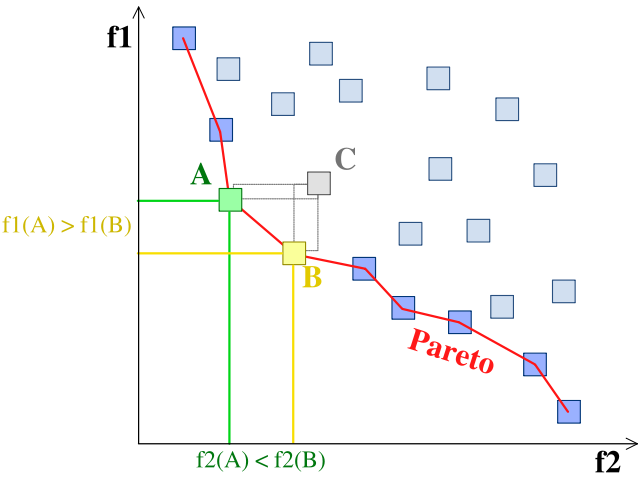
\includegraphics[width=0.5\textwidth]{pareto.png}
    \caption{Beispiel einer Pareto-Front \cite{Paretofr62:online}}
    \label{fig:pareto}
\end{figure}

Eine beispielhafte Darstellung der Pareto-Front zeigt \autoref{fig:pareto}.
$f1$ ist z.B. die Fitness der Anzahl und $f2$ die Fintess der Strecke.
In diesem Programmentwurf lässt sich mittels der GEwichtung steuern,
in welchem Bereich der Pareto-Front eine Lösung gesucht wird.
Je stärker die Anzahl gewichtet wird, desto weiter Links befindet sich die Lösung in diesem Schaubild.

\newpage
\section{Prototyp}\label{sec:prototyp}

Der diesem Programmentwurf angehängte Prototyp basiert grundlegend auf der Implementierung in \cite{Quiz15Th91:online}.
Diese Implementierung löst das Knappsackproblem mit Hilfe eines Genetischen Algorithmus.
Sie wurde auf die hier beschriebenen Methoden angepasst und unter anderem
in diesen Punkten geändert:
\begin{itemize}
    \item Eingabe der Daten über eine wohlgeformte CSV-Datei anstatt einer unübersichtlichen Textdatei.
    \item Entfernen der ungültigen Gene aus der Population anstatt sie \enquote{nur} mit einer Fitness von $0$ zu versehen.
    \item Anpassung der initialen Population
\end{itemize}


\noindent
Zur Validierung des Prototyps stehen Testdaten zur Verfügung.
Die Orte der Testdaten entstammen aus tatsächlichen Spende-Orten in einem Umkreis von 25 km um einen bestimmten Ort.
Da lediglich Daten bis Mitte Dezember 2018 vorliegen,
werden für die Testdaten zufällige Termine für das Jahr 2019 erzeugt.

In den nächsten Unterabschnitten wird der Verlauf verschiedener Werte während eines Durchlaufes betrachtet.
Hierzu wird das Programm mit folgenden Parametern ausgeführt:
\begin{table}[ht]% Try here, and then top
    \begin{center}
        \begin{tabular}{l|c}
            Parameter                       & Wert \\
            \hline
            Population                      & $500$  \\
            Maximale Iterationen            & $1000$ \\
            Anteil der Elite                & $20\%$ \\
            Mutationswahrscheinlichkeit     & $80\%$ \\
            Initiale Schrittweite           & $3$     \\
            Präzision für Stoppbedingung  & $10^{-4}$
        \end{tabular}
    \end{center}
    \caption{Parameter}
    \label{tab:parameter}
  \end{table}


% Echte Daten von:
% https://www.blutspende.de/infos-zur-blutspende/blutspende-termine/blutspendetermine.php?umkreis=25&abgeschickt=1&plz_ort_eingabe=74076&d_v_eingabe=13.09.2018

\subsection{Entwicklung der Fitness}

Führt man den Prototypen mit den Testdaten aus,
 so lässt sich für die Fitnesswerte die Entwicklung in \autoref{fig:fitness} beobachten.
Zwar fällt die schlechteste Fitness nach der initialen Generation ab,
aber sowohl die durchschnittliche, als auch die beste Fitness steigen an.
Dies bedeutet, dass zwar mindestens ein Gen mit einer schlechteren Fitness entsteht,
jedoch insgesamt \enquote{bessere} Gene erzeugt werden.

Der beste und der durchschnittliche Fitnesswert konvertieren gegen ca. $0,953$.
Dies ist auch das in diesem Durchlauf erreichte Optimum.
Das beste Gen erreicht diesen Wert bereits in der siebten Generation.

Die schlechteste Fitness fällt nach der initialen Generation ab,
steigt aber wieder an und konvergiert zunächst gegen ca. $0,82$,
macht jedoch in der letzten Generation einen Sprung zu ca. $0,953$.
Wahrscheinlich werden in dieser Generation die verbleibenden \enquote{weniger guten} Gene durch das beste gefundene Gen verdrängt.

\begin{figure}[ht]
    \centering
    \begin{tikzpicture}
        \begin{axis}[
            reverse legend,
            xlabel={Generation},
            ylabel={Fitness},
            legend pos=south east,
            width=12cm,
            height=7.41cm,
            enlarge x limits=false,
            enlarge y limits=false,
            ymin=0,
            ymax=1
        ]
        \addplot[mark=*,LineRed] plot coordinates {
            (0,0.39809812568908487)
            (1,0.3137908857037854)
            (2,0.35191106210951856)
            (3,0.43761944138184494)
            (4,0.4597023153252481)
            (5,0.5794377067254686)
            (6,0.6075523704520397)
            (7,0.697827085630283)
            (8,0.7221536199926498)
            (9,0.8083664094083058)
            (10,0.8288239617787578)
            (11,0.8288239617787578)
            (12,0.9531284454244763)
        };
        \addlegendentry{Schlechteste Fitness}
        \addplot[mark=diamond*,LineBlue] plot coordinates {
            (0,0.5010904812526614)
            (1,0.533322685651329)
            (2,0.5815548190310615)
            (3,0.6395867099505065)
            (4,0.700842131783521)
            (5,0.7559416493970084)
            (6,0.8170118889289913)
            (7,0.870926735946039)
            (8,0.9198439253202729)
            (9,0.9420204083027279)
            (10,0.9454525511769829)
            (11,0.9520316362842004)
            (12,0.9531284454244685)
        };
        \addlegendentry{Durchschnittliche Fitness}
        \addplot[mark=triangle*,LineGreen] plot coordinates {
            (0,0.6075248070562294)
            (1,0.7140963800073502)
            (2,0.7776552737963984)
            (3,0.8356045571481074)
            (4,0.8917998897464168)
            (5,0.9459619625137817)
            (6,0.9459619625137817)
            (7,0.9531284454244763)
            (8,0.9531284454244763)
            (9,0.9531284454244763)
            (10,0.9531284454244763)
            (11,0.9531284454244763)
            (12,0.9531284454244763)
        };
        \addlegendentry{Beste Fitness}
        \end{axis}
    \end{tikzpicture}
	\caption{Fitnesswerte der verschiedenen Generationen}
	\label{fig:fitness}
\end{figure}

Interessanterweise sind in der zwölften Generation
die Fitnesswerte des besten und des schlechtesten Gens identisch mit $0,9531284454244\highlight{lime!30}{763}$.
Der Gesamtdurchschnitt wird jedoch lediglich mit $0,9531284454244\highlight{lime!30}{685}$ angegeben.
In den letzten drei Ziffern ist der Durchschnitt also geringer als das Minimum.
Mathematisch ist dies zwar unmöglich, kann aber auf numerische Fehler bei der Berechnung zurückgeführt werden.

Daraus, dass in der letzten Generation sowohl Minimum und Maximum die gleiche Fitness haben,
als auch alle Gene die Bedingungen erfüllen kann geschlossen werden, dass in dieser Generation alle Gene identisch sind.
Somit endet der Algorithmus sinnvollerweise an dieser Stelle.

\subsection{Entwicklung gültiger Gene}

\autoref{fig:ueberlebende} zeigt die Anzahl der gültigen Gene im Verlauf der Generationen.
In der initialen Generation erfüllen lediglich $391$ Gene - etwa ein 78\% - die gestellten Bedingungen.
Von Generation $1$ bis $8$ schwank diese Zahl zwischen $452$ und $461$ um dann zu steigen,
 bis in Generation $12$ alle Gene gültig sind.

\begin{figure}[ht]
    \centering
    \begin{tikzpicture}
        \begin{axis}[
            legend pos=south east,
            enlarge x limits=false,
            enlarge y limits=false,
            width=12cm,
            height=7.41cm,
            ymin=375,
            ymax=500
        ]
        \addplot[
            name path=B,
            LineGreen,
            mark=*
            ] coordinates {
            (0, 391)
            (1, 461)
            (2, 449)
            (3, 454)
            (4, 446)
            (5, 432)
            (6, 446)
            (7, 436)
            (8, 452)
            (9, 484)
            (10,485)
            (11,498)
            (12,500)
        };
        \end{axis}
    \end{tikzpicture}
	\caption{Anzahl gültiger Gene}
	\label{fig:ueberlebende}
\end{figure}

\newpage
\subsection{Entwicklung der Mutationsrate}

In \autoref{fig:mutationsrate} wird die Entwicklung der Mutationsrate dargestellt.
Der Anstieg in den ersten beiden Generationen und spätere Rückgang zeigt,
dass gerade am Anfang durch Mutationen eine deutliche Verbesserung der Gene erreicht werden kann.
Gegen Ende nimmt diese Verbesserung ab. Hieraus lässt sich auf ein (lokales) Optimum schließen.

\begin{figure}[ht]
    \centering
    \begin{tikzpicture}
        \begin{axis}[
            legend pos=south east,
            enlarge x limits=false,
            enlarge y limits=false,
            width=12cm,
            height=7.41cm,
            ymin=0,
            ymax=5
        ]
        \addplot[
            LineBlue,
            mark=*
            ] coordinates {
            (0, 3)
            (1, 4)
            (2, 5)
            (3, 4)
            (4, 3)
            (5, 2)
            (6, 1)
            (7, 1)
            (8, 1)
            (9, 1)
            (10,1)
            (11,1)
            (12,1)
        };
        \end{axis}
    \end{tikzpicture}
    \caption{Mutationsrate}
    \label{fig:mutationsrate}
\end{figure}


\newpage
\section{Fazit}\label{sec:fazit}
\blindtext

%\printacronyms{}
\newpage
\printbibliography{}
\end{document}
